\section{Commercial LCR meters} \label{sec:CommercialLCRMeters}
Most of the major manufacturers of test equipment, such as Keysight Technologies, Rohde \& Schwarz, Tektronix and others produce a range of instruments for characterizing passive components. This section will review a few of these to find out what their capabilities are. 

LCR meters typically come in two different form factors, one is a handheld device, much like a regular multimeter, while the other is a benchtop instrument. The handheld LCR meters, like the Keysight U1733C\cite{KeysightU1733C} shown on figure \ref{fig:2_2_U1733C}.
\begin{figure}[H]
    \centering
    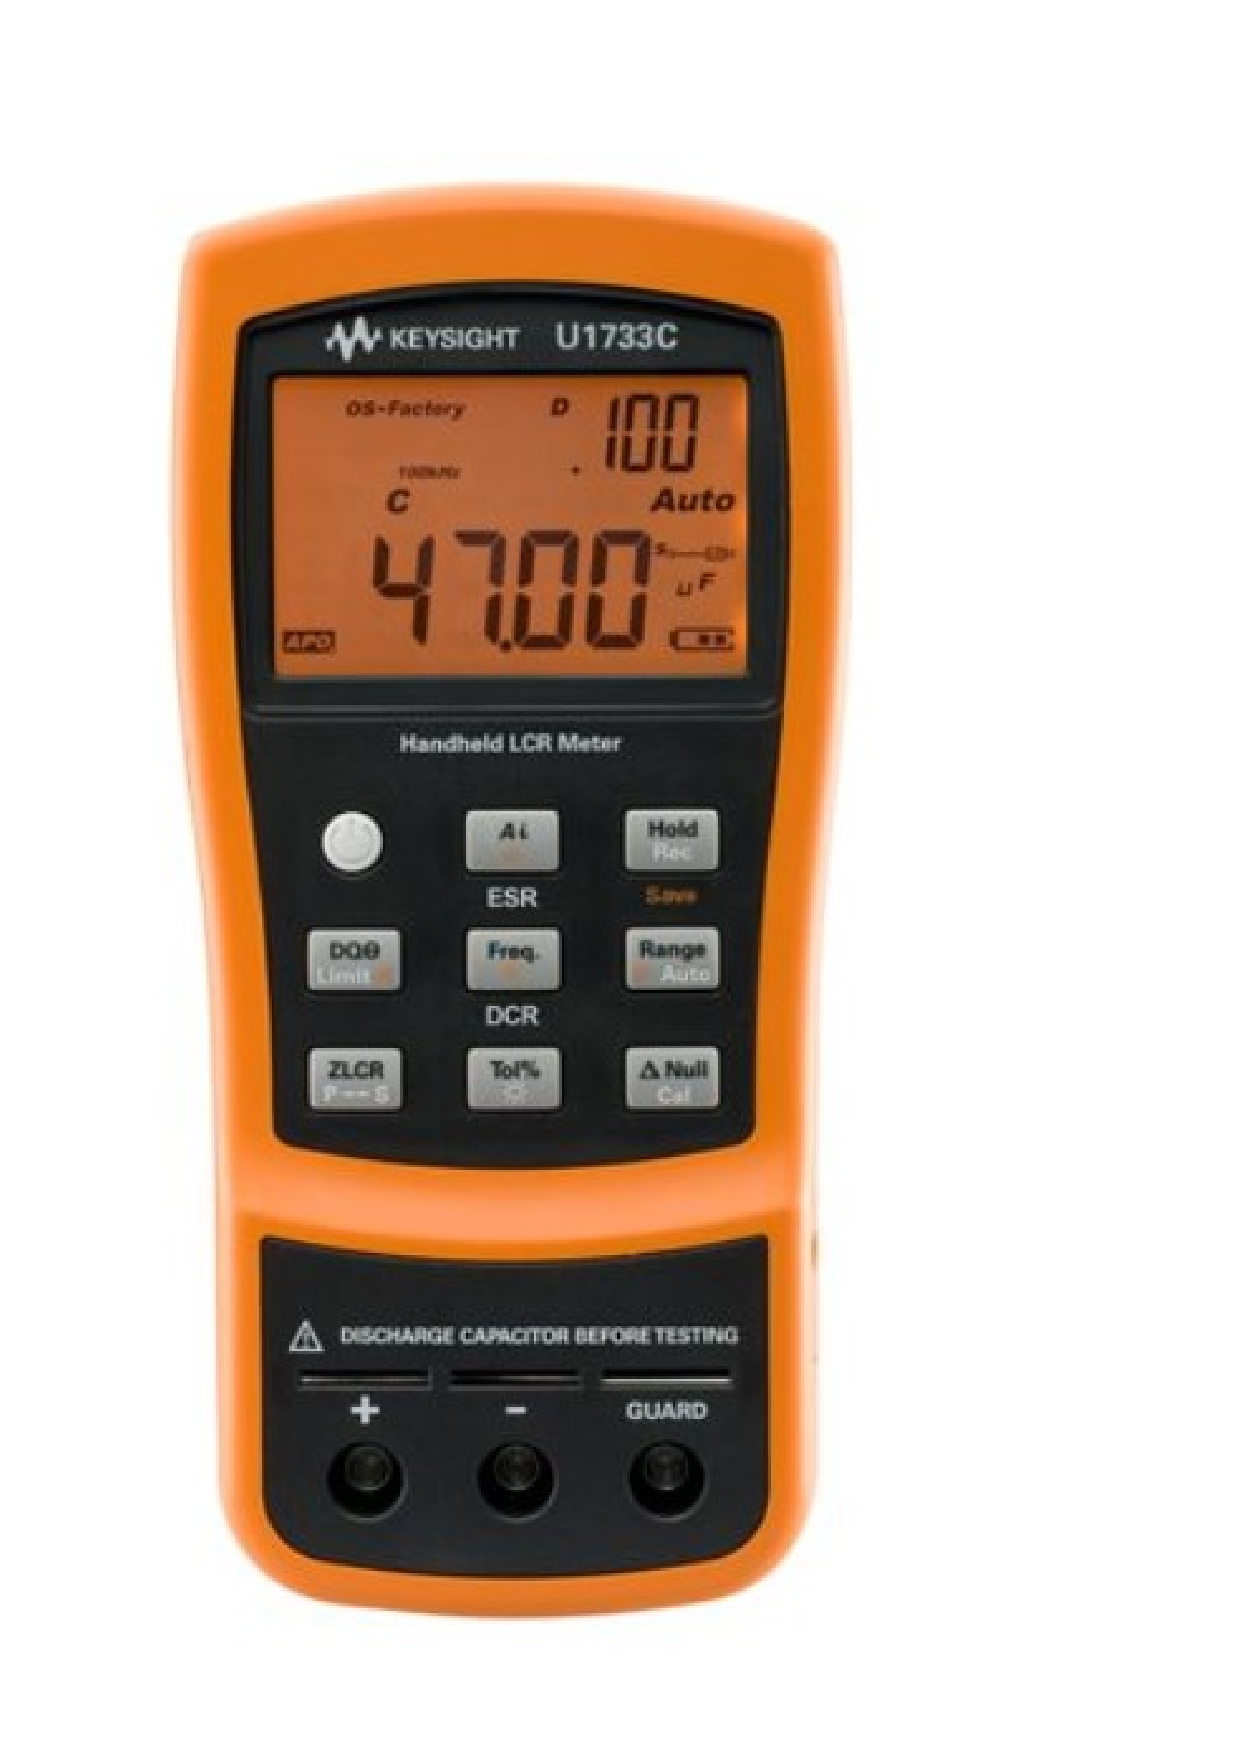
\includegraphics[clip, trim=0 50 0 50, width=0.5\textwidth]{Sections/2_ProblemAnalysis/FIgures/KeysightU1733C.pdf}
    \caption{A handheld Keysight U1733C LCR meter.}
    \label{fig:2_2_U1733C}
\end{figure}
The U1733C \ref{fig:2_2_U1733C}, while affordable at about 550€, has limited capabilities. It can measure all the basic parameters such as capacitance, inductance, ESR and display all the derived quantities like dissipation and quality factor, however it can only take these measurements at pre-determined test frequencies in the range \SI[]{100}{\hertz} to \SI[]{100}{\kilo\hertz} 




%Vi kigger kun på bord LCR metre

%VI kigger på 3 forskellige
%Keysight
%RS
%Tek

%De har xyz specs og kan de her ting.

%De er beregnet til xyz

%de koster xyz

